\section{Carmichael-Funktion}

Die Carmichael-Funktion $\lambda(n)$ gibt für eine natürliche Zahl $n$ die kleinste positive ganze Zahl an, sodass für alle zu $n$ teilerfremden Zahlen $k$ gilt:

\begin{align}
  k^{\lambda(n)} \equiv 1\pmod{n}
\end{align}

Die Funktion kann wie folgt definiert werden:

\begin{align}
  \lambda(n) = \operatorname{kgV}\left[(p_i-1)p_i^{a_i-1}\right]_i
\end{align}\cite{mw04}

Hierbei steht $p_i$ für den i-ten Primfaktor von $n$ und $a_i$ für den Exponent des i-ten Primfaktores.\cite{mw05}

Um $\lambda(n)$ einer Zahl zu berechnen werden folgende Schritte verwendet:

\begin{enumerate}
  \item Zahl in Primfaktoren zerlegen
  \item Alle Primfaktoren in $(p_i-1)p_i^{a_i-1}$ einsetzen und die Ergebnisse speichern
  \item den kleinsten gemeinsamen Teiler aus allen Ergebnissen bilden
\end{enumerate}

Beispielhalft sei $n$ gleich $15$:

\begin{equation}
  \begin{aligned}
    n&=15=3^1 \cdot 5^1 && \text{Darstellung durch Primfaktoren}\\
    p_0&=3 && \text{Erster Primfaktor von $15$}\\
    p_1&=5 && \text{Zweiter Primfaktor von $15$}\\
    a_0&=1 && \text{Exponent des ersten Primfaktors $3$}\\
    a_1&=1 && \text{Exponent des zweiten Primfaktors $15$}\\
    k&=\left((p_0 - 1) \cdot p_0^{a_0 - 1};\, (p_1 - 1) \cdot p_1^{a_1 - 1}\right) && \text{Folge $k$ welche Ergebnisse enthält}\\
    \hookrightarrow&=\;\,((1;\, 12))\\
    \lambda(15)&=\operatorname{kgV}(k)=4
  \end{aligned}
\end{equation}

Oder für $n \in \mathbb{P}$:

\begin{equation}
  \begin{aligned}
    n&=17=17^1 && \text{Nur 1 und 17 als Primfaktor, da prim}\\
    p_0&=17\\
    a_0&=1\\
    k&=((17-1) \cdot 17^{1-1})\\
    \lambda(17)&=\operatorname{kgV}(k)=16
  \end{aligned}
  \label{carmichael:prime}
\end{equation}

die Berechnung in \ref{carmichael:prime} zeigt einen Sonderfall der Carmichael-Funktion, denn für alle $n \in \mathbb{P}$ ist $\lambda(n)=n-1$, wie in \ref{carmichael:primes} weiter zu sehen ist.

\begin{equation}
  \begin{aligned}
    \lambda(2)&=1\\
    \lambda(3)&=2\\
    \lambda(5)&=4\\
    \lambda(7)&=6\\
    \lambda(11)&=10\\
    \lambda(13)&=12\\
    ...&
  \end{aligned}
  \label{carmichael:primes}
\end{equation}

Abbildung \ref{carmichael_dist} zeigt die Verteilung von $\lambda(n)$ für die ersten eintausend Werte $n$. Abbildung \ref{carmichael_totient} zeigt eine kombinierte Verteilung von sowohl der eulerschen Phi-Funktion als auch der Carmichael-Funktion.

\begin{figure}[H]
  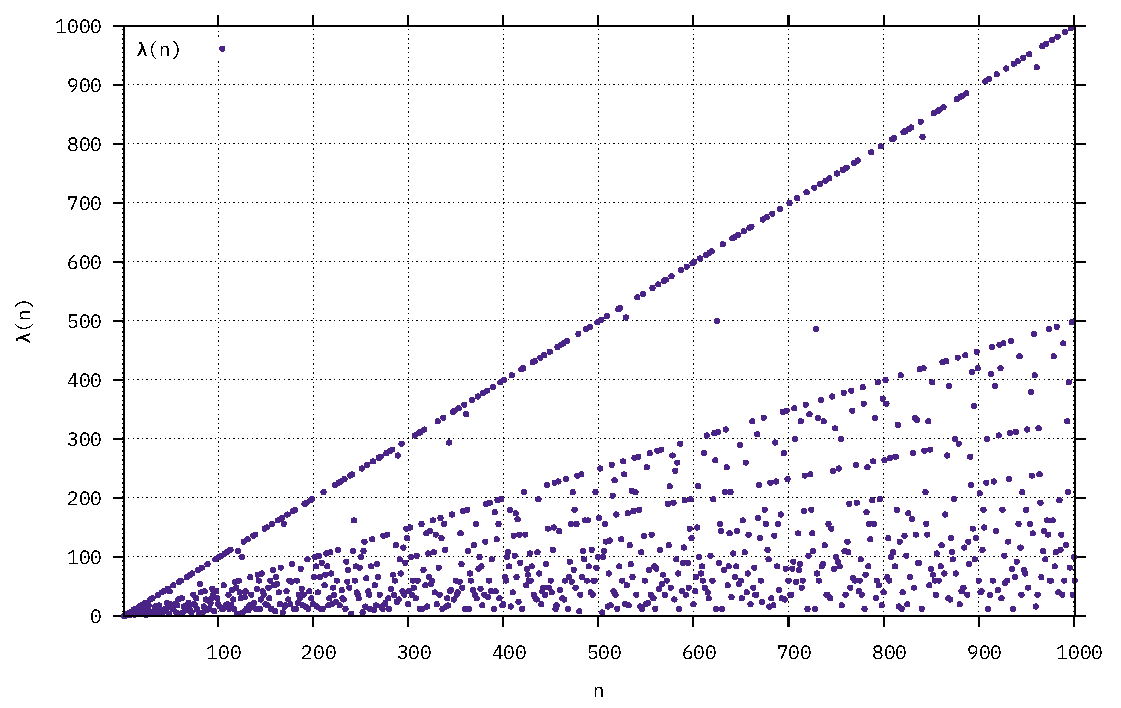
\includegraphics{carmichael.pdf}
  \caption{Carmichael-Funktion $\lambda(n)$ für $\left\{\,n \in \mathbb{N}\mid 1 \le n \le 1001 \, \right\}$}
  \label{carmichael_dist}
\end{figure}

\begin{figure}[H]
  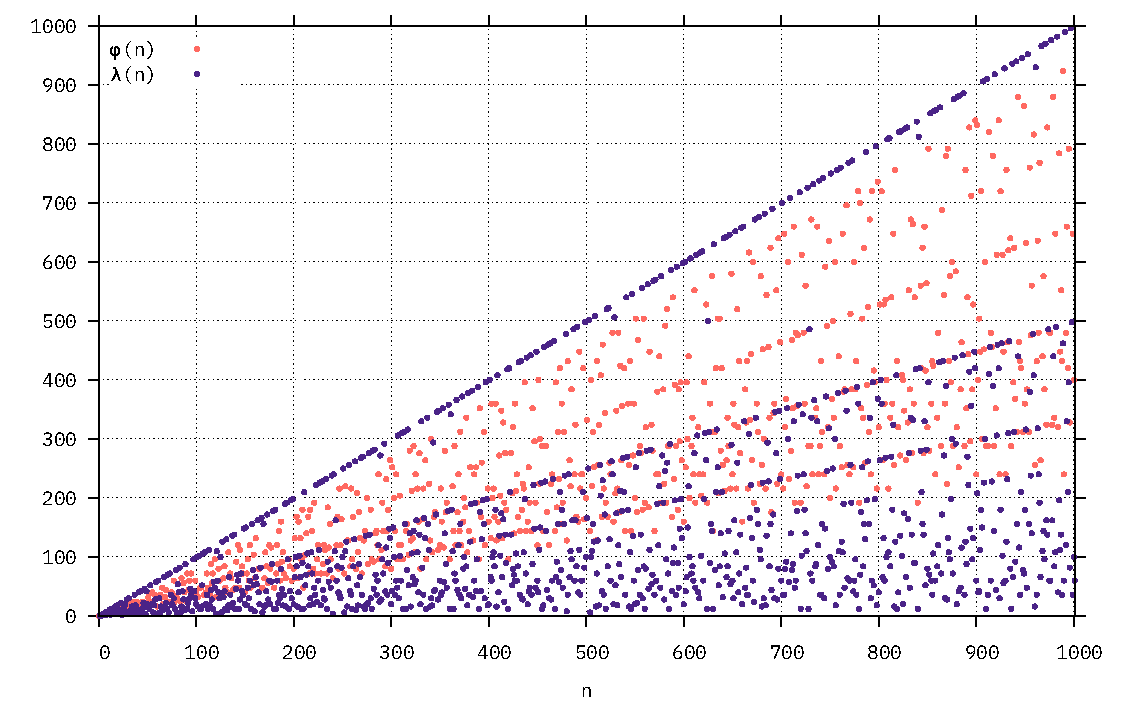
\includegraphics{totient_carmichael.pdf}
  \caption{Carmichael-Funktion $\lambda(n)$ für $\left\{\,n \in \mathbb{N}\mid 1 \le n \le 1001 \, \right\}$ und eulersche Phi-Funktion $\varphi(n)$ für $\left\{\,n \in \mathbb{N}\mid 0 \le n \le 1000 \, \right\}$}
  \label{carmichael_totient}
\end{figure}
